\documentclass{utue} %utue.cls required for Uni Tuebingen corporate design

% Values for title generation
\title{Reading scene text in deep convolutional sequences}
\author{Jan Haug, Marius Hobbhahn, Roman Schulte}
\date{\today}

% Subtitle is optional. It represents what kind of work you did.
\subtitle{Winter Term 2017}

\begin{document}

% You can place a teaser as follows. (Otherwise, just uncomment the following part)
\teaser{
    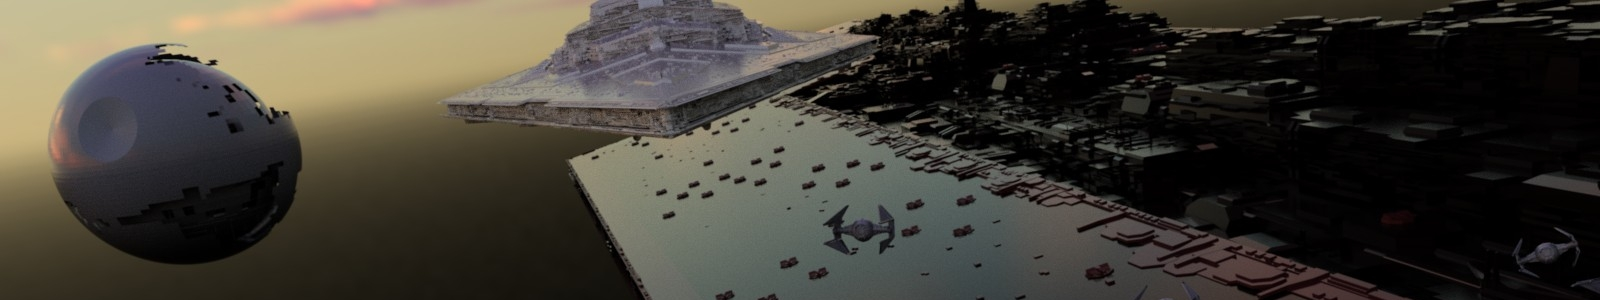
\includegraphics[width=\textwidth]{images/teaser.jpg}
    \caption{\label{fig:teaser}You can place a teaser here.}
}

% Creates title of document and additional title page.
\maketitle

\section*{Abstract}

\section{Introduction}

Natural scene recognition is one of the most important tasks in numerous automation processes. Autonomous cars have to be able to identify construction signs to follow their instructions, traffic agencies can identify license plates of traffic offenders %citation of license plate paper
and robots will need to read text and numbers in a natural environment. In 2015, He et. al ~\cite{2015arXiv150604395H} proposed a model to read scene text in natural environments with a combination of a convolutional neural network (CNN) and recurrent neural network (RNN) which is not restricted to having words pre-defined in a dictionary or segmentation of individual letters (which poses a difficult task by itself), but instead views the input as a sequence and uses context information to decode a word as a whole, e.g. on an advertisement sign. One of the main challenges of scene recognition is the high variance in image quality and style of displayed signs. The same word can be represented in many different ways in an image by variation in lighting, colours, perspective or font. The approach chosen by the authors has some advantages over previous approaches (i.e. %citation of previous approaches
), which fail to capture all representations of strings in a natural environment. It uses a combined model, capitalizing on both the high performance in character recognition of CNNs and also the ability of RNNs to process context information in sequences. \\
\begin{enumerate}
	\item CNNs have become very accurate at character recognition and building high level representations. 
	%citation if possible.
	By moving a sliding window over a given picture, we are able to create character-level inputs without concerns about character segmentation, as this problem is handled by the RNN part of the model. The simplicity of a sliding window approach implies that some frames will not yield beneficial results, but the RNN is also able to process unclear outputs of the CNN; this only means that the sliding window should be moved in small steps, so no characters can be skipped by accident. On the other hand, this simplicity results in not only a small (i.e. fast) CNN, but also in a high versatility, as the inputs do not need to be pre-processed except for the trimming around a word and the re-scaling to a 32px height.
	\item RNNs are very strong at processing sequences of inputs and accounting for context information, especially when the length of a given sequence is unknown at first.
	%citation if possible.
	As words are nothing else than sequences of letters (with variable length), the application of an RNN seems very intuitive. Due to this context information, the RNN can make decisions for a sign based on the previously identified signs, i.e. The letter 'a' might be more likely to occur after a 'b' than an 'y'. Since the RNN receives the activations of the penultimate layer of the CNN (which has more neurons), there should also be more information on letters in direct vicinity to the recognized one, since there will usually be more than one symbol in the sliding window. To use context information from previous and later signs we use a bidirectional approach, that independently applies the model forwards and backwards. 
	\item If property 1 and 2 are combined successfully, it is possible to process unknown words and arbitrary sequences of symbols. Since the training is done in a compositional way, it is independent of dictionaries or corpora of already known words and combinations of strings. Therefore it would be able to read the information on any given picture even if no meaning is attached to it. The only restriction is that the set of symbols needs to be specified as the CNN classifies each input as one of 26 letters or of the 10 different digits (i.e. the recognition of special letters like Umlauts would require slight modifications to the model and retraining it from scratch)
\end{enumerate}
The main contribution of this paper was to improve the accuracy in scene text recognition on given benchmark test sets like the IIIT5K.%citation (should be on their website)
Our contribution is the attempt to reproduce the work of the paper, the comparison of the results given the same benchmarks, and the documentation of possible caveats or other difficulties during this process, especially where the authors do not specify details on the implementation or its parameters.

\section{Related Work}
%don't just copy papers from the original paper, but look for more recent ones, i.e. 2016/17
%describe the research goal of the other paper, the differences to our approach and why this difference is important here
% this is the citation of the main paper ~\cite{2015arXiv150604395H} 
% probably should choose better citation style, mache ich ~Jan
The paper in discussion was written by He et al. from 2015 ~\cite{2015arXiv150604395H}. In this section we would like to address two types of related papers. Firstly, papers that have tried different approaches to solve the same task but with less accurate results. These will be mainly papers published before the original paper. Secondly, we explore how the presented methods was applied to other related tasks in later publications. Follow up studies and improvements will be provided in the discussion part of this paper. \\
%papers before ours
Earlier approaches of text scene recognition like shown in ~\cite{Mishra2012a} , or ~\cite{6727574} used combinations of structure guided character recognition, linguistic knowledge and Bayesian inference via decision trees. All of these broke the benchmarks on frequently used data sets such as IIT5K or ICDAR but did not use learning algorithms based on neural networks. First approaches of leveraging the advantages of neural networks were done for example by ~\cite{DBLP:journals/corr/AlsharifP13}, who used a classical CNN and hybrid hidden Markov models (HMMs), which could be seen as predecessors of the frequently used connectionist temporal classification (CTC) of today, which is also used in the final part of the model presented here.
%papers with different goal
The very same model idea as described here, i.e. a combination of sliding window, CNN, RNN and CTC, was used to significantly improve benchmarks for other tasks of scene recognition. ~\cite{DBLP:journals/corr/GuoTLL16} for example used the method for the recognition of house numbers and achieved an accuracy of 91 percent, compared to 81 percent of previous approaches. ~\cite{DBLP:journals/corr/LiS16} were able to lift the benchmark of license plate recognition on the Caltech cars data set from 95.5 to 97.56 and the recall from 84.8 to 95.24 percent. The difference between precision and recall in this paper not only implies superior recognition if the plate has been detected but also superior detection of license plates in the first place. Both of these papers show the strength of the combining CNN and RNN in a single model. The way~\cite{2015arXiv150604395H} differs from these approaches is through very high diversity of the image inputs: License plates and house numbers have much more structure and in the house number case, less different symbols on it. With the IIIT5K dataset, the network can make far fewer assumptions about its inputs, since there are a lot of different shapes within each class due to the vast amount of different fonts used.


\section{Structure of the network}
%just the theory behind the network
After applying a sliding window on a given image each frame is forwarded into a CNN. The sequence of resulting feature vectors is then sent through the RNN and results in a sequence of characters and numbers. An overview of the whole network is given in graphic \ref{fig:model_general}

\begin{figure}[h!]
	\centering
	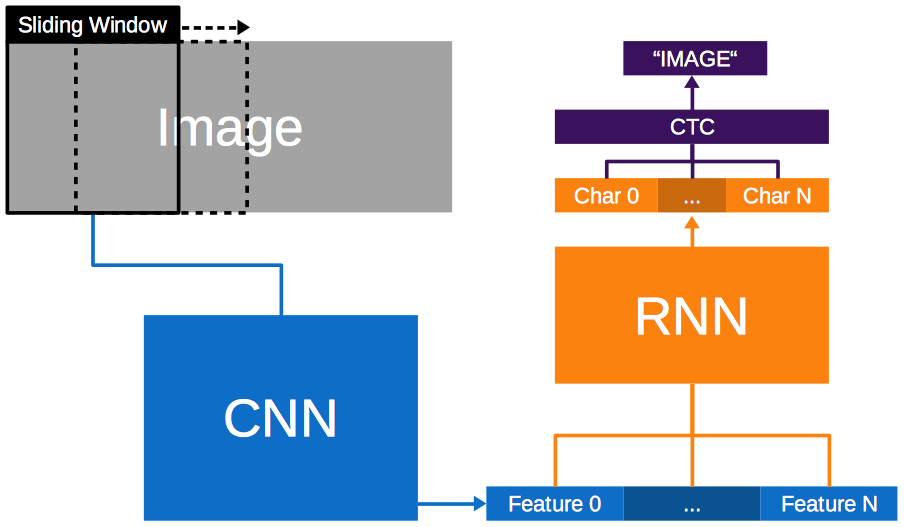
\includegraphics[width=.9\columnwidth]{graphics/model_general.png}
	\caption{\label{fig:model_general} \footnotesize{structure of the whole network with sliding window, CNN, RNN and CTC.}}
\end{figure}

\subsection{Data wrangling}
We rescale the image to height 32 and then apply a sliding window of framesize 32x32 for every 8 pixels of length. When reaching the end of the image we adjust the current frame such that the last frame is 32x32 and includes the column of pixels on the right edge of the image. A graphical interpretation of the process can be seen in figure \ref{fig:sliding_window}

\begin{figure}[h!]
	\centering
	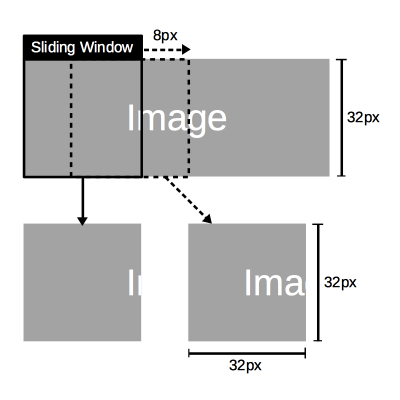
\includegraphics[width=.9\columnwidth]{graphics/model_sliding_window.png}
	\caption{\label{fig:sliding_window} \footnotesize{a graphical depiction of the sliding window.}}
\end{figure}


\subsection{Structure of the CNN}
The CNN has 5 convolutional layers. In the first 3 we apply a 9x9 kernel on the inputs and use a max. group of 2. For the 4th layer a 8x8 kernel and a max group of 4 is used to reduce the dimensionality of the output vector to 128. Note that this output of a 128D feature vector is forwarded into the RNN. The 5th layer uses a 1x1 kernel %is this equivalent to no kernel?
and also uses a max group of 4 to further reduce dimensionality. This output is then forwarded through a fully connected layer with 36 outputs for the 26 possible lower case characters and 10 numbers. For activation we use the identity function. Note that the last convolutional and the fully connected layer are merely used for the training of the CNN but later not used for the classification in the RNN. A detailed description of the network can be seen in graphic \ref{fig:cnn_structure}.

\begin{figure}[h!]
	\centering
	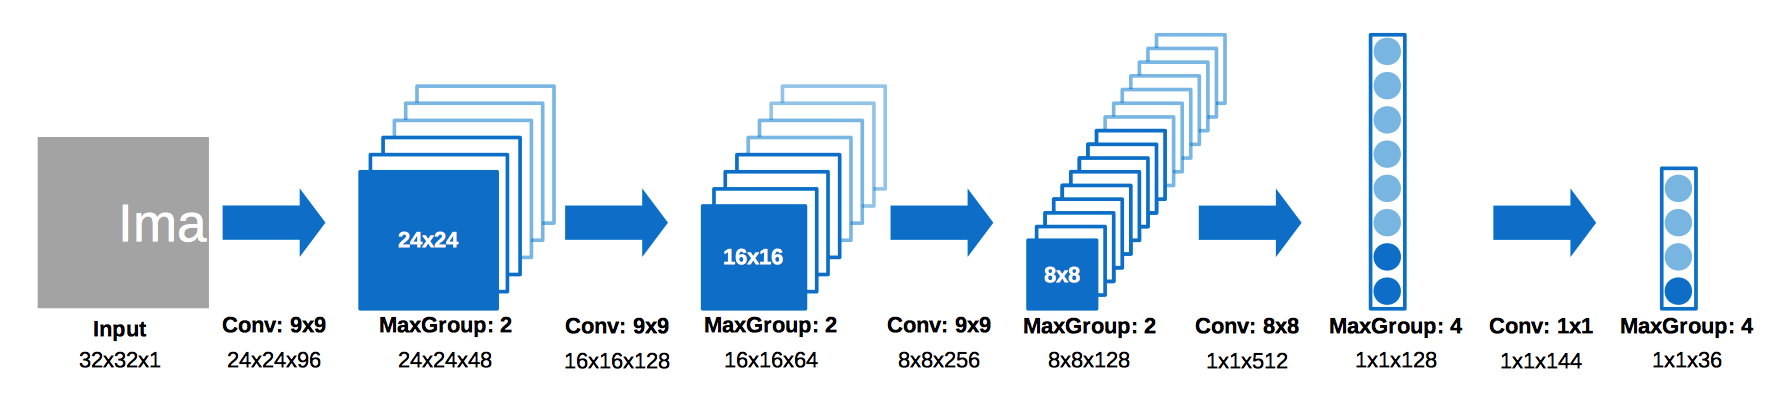
\includegraphics[width=.9\columnwidth]{graphics/model_cnn.png}
	\caption{\label{fig:cnn_structure} \footnotesize{structure of the CNN with 5 convolutional layers and 1 fully connected on top.}}
\end{figure}

\subsection{Structure of the RNN}
The recurrent part of the network receives a sequence of feature vectors, each of which is provided by the CNN. We use bidirectional stacked long-short-term-memory (LSTM) cell blocks with 128 inputs respectively as developed by ~\cite{Hochreiter:1997:LSM:1246443.1246450} originally. Bidirectional means that the RNN essentially has 2 independent units. In one the sequence is put in forwards and the other backwards. The results are then concatenated afterwards and fed into a fully connected layer with 37 output classes. 26 for each character 10 for numbers and 1 for undetectable sign or no character. This can be seen in figure \ref{fig:rnn_structure}. \\
\begin{figure}[h!]
	\centering
	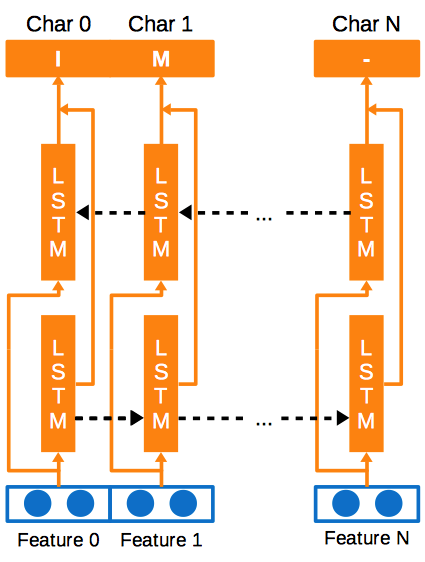
\includegraphics[width=.9\columnwidth]{graphics/model_rnn.png}
	\caption{\label{fig:rnn_structure} \footnotesize{structure of the RNN with a bidirectional approach with 128 inputs respectively.}}
\end{figure}

At this point we still have redundancies or unclear information due to the sliding window. To solve this problem a connectionist temporal classification (CTC) is used. A detailed explanation would be outside of the scope of this paper and can be found in the original paper  ~\cite{Graves:2006:CTC:1143844.1143891}.
But for a working explanation consider it as a way to remove unlikely information given the labels. In sequential information the placement of non-character symbols or redundancies is always hard to deal with. The CTC approach therefore uses a hidden Markov model (HMM) to sample different possible outcomes as paths in a tree and choose the path with highest likelihood. Consider an example where the sequence after the LSTM cell block is "iiii---mmmmaaagggee--", where - represents the non-character symbol. The CTC would then reduce the redundancies and remove non-character symbols until the most likely outcome, "image" is put out. The information learned by the CTC during the training are backpropagated through the network such that future classification can already access them. A graphical overview is provided by figure \ref{fig:structure_ctc}. \\

\begin{figure}[h!]
	\centering
	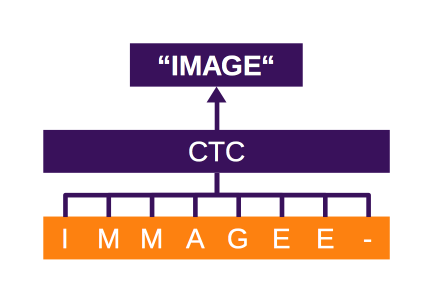
\includegraphics[width=.9\columnwidth]{graphics/model_ctc.png}
	\caption{\label{fig:structure_ctc} \footnotesize{very simplified structure of the CTC.}}
\end{figure}

\section{Implementation details}
%here are the names of functions, comparisons with other possible implementations and numbers (i.e. number of epochs, momentum terms, learning rates, etc. )
\subsection{Data wrangling}
TODO
\paragraph{Sliding window}
\paragraph{Batch sizes}
TODO %I only inserted the graphic, explanaition at best done by roman

figure \ref{fig:impl_rnn_labels}.
\begin{figure}[h!]
	\centering
	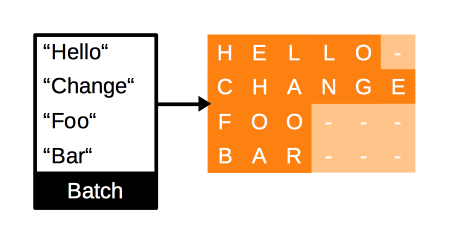
\includegraphics[width=.9\columnwidth]{graphics/impl_rnn_labels.png}
	\caption{\label{fig:impl_rnn_labels} \footnotesize{implementation of batchsizes for the training of the RNN.}}
\end{figure}


\subsection{Implementation details of the CNN}
The convolutional layer were implemented using the conv2D() function provided by the tensorpack library and combined with a self-made maxgroup() function, since the tensorflow version had an error. The functionality of athe maxgroup can be seen in figure \ref{fig:impl_maxgroup}. Instead of a softmax in the end, like in the original paper, we chose a fully connected layer with identity as activation function since it lead to a higher accuracy for the character recognition. \\
\begin{figure}[h!]
	\centering
	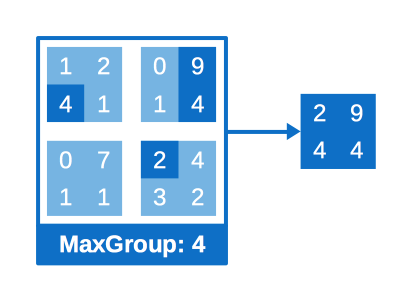
\includegraphics[width=.9\columnwidth]{graphics/impl_maxgroups.png}
	\caption{\label{fig:impl_maxgroup} \footnotesize{functionality of the self-made maxgroup function.}}
\end{figure}

For the training we use a learning rate with exponential decay starting at 0.001 with decay rate of 0.99 and getting smaller every 5 epochs. As an optimizer we chose the AdamOptimizer() and used the prebuild InferenceRunner() from tensorpack to check for validation accuracy on a test set and prevent overfitting. Overall we train for 1500 epochs and use the prebuild SimpleTrainer() from tensorpack. 

\subsection{Implementation details of the RNN}
The RNN is implemented using the prebuild tensorflow functions tf.nn.bidirectional\_dynamic\_rnn with tf.nn.BasicLSTMCell for both directions. We use 128 units as described in the original paper and a tanh as activation function. For the fully connected layer on top we use tf.contrib.layers.fully\_connected with identity as activation. \\
%this text is really redundant so far
The CTC exists prebuild as well. For the loss we use the tf.nn.ctc\_loss and tf.nn.ctc\_greedy\_decoder for the model. The greedy decoder is a variant of the tf.nn.ctc\_beam\_search\_decoder function that is faster but less accurate. For our training the beam search decoder was too slow and in comparison did not add any visible improvements during the first couple of steps in training which lead us to using the greedy decoder.  \\
For the training we use the Adam optimizer with a learning rate of 0.0001 and a momentum term of 0.9 over 1500 epochs. Since we divided our data set in test and train split we also use the InferenceRunner() class provided by the tensorpack library to prevent overfitting and check for validation accuracy. 

\section{Experiments and Results}
%detailed description of what datasets we were using, what the results of the singular training for the CNN were, what the results for the RNN were
%explanation of the inference runner, test error and validation accuracy
The test images solely came from the openly available IIT5K data set. In the original study two other set of images were additionally used but seemed to only contribute very small amounts of images. So only using the IIT5K seemed sufficiently justifiable in this case. As the name suggests we initially have 5000 images of which a small amount was sorted out since they did not have 32 pixels in width. After segmentation the CNN trains on %insert number of labeled 32x32 pictures
labeled 32x32 pictures and the RNN on around 2500 pictures with scene text due to the test train split. 
The experiments were conducted on the just described data sets using the training details listed in the respective implementation details section. \\
The CNN converges against an accuracy of 0.97 on the training set with a validation accuracy of 0.62. The process can be viewed in graphic  \ref{fig:cnn_accuracy}.\\

\begin{figure}[h!]
	\centering
	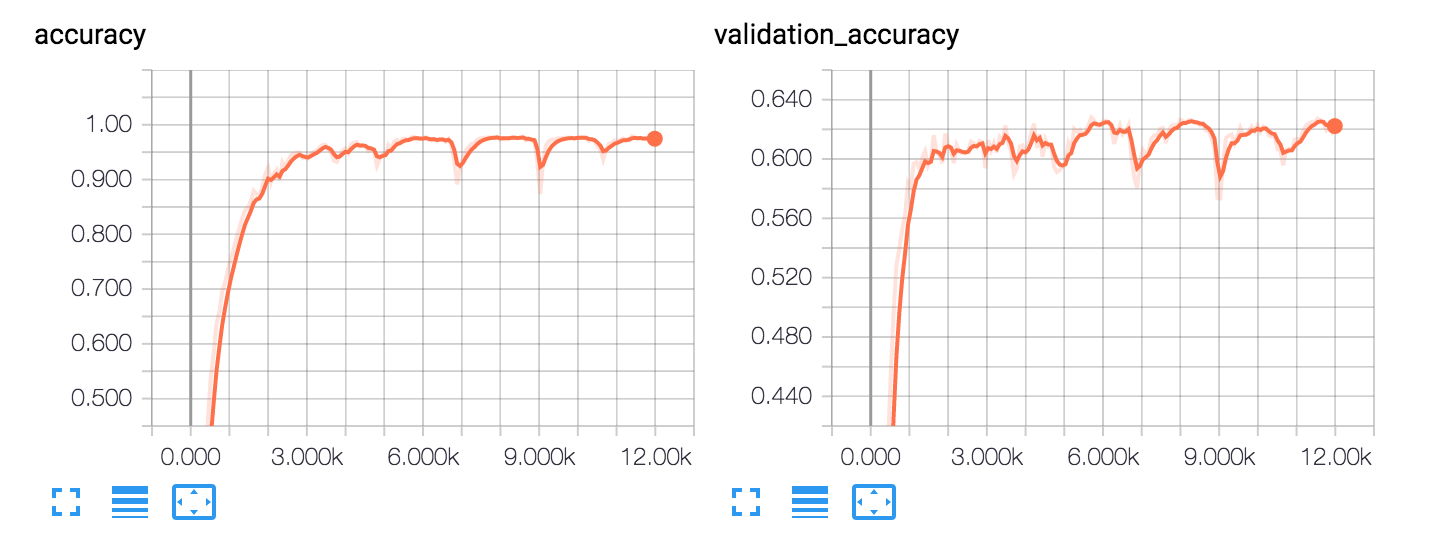
\includegraphics[width=.9\columnwidth]{graphics/cnn_accuracy.png}
	\caption{\label{fig:cnn_accuracy} \footnotesize{training process for the CNN. Training accuracy on the left and validation accuracy on the right.}}
\end{figure}

The validation accuracy seems rather low for a task like character recognition. This might be due to overfitting, very unclear images or just a suboptimal model. But note that the 5th and 6th layer of the CNN never get used at later stages anyways so only the accuracy of the 128D feature vectors matters. This can not be determined directly but only through the loss of the RNN at later stages. \\
The RNN converges against an accuracy of 1 on the training set and against 0.66 for the validation. Note here that this is an increase compared to the 0.62 of the CNN solely, meaning the context of the word significantly added to identification of the letters. Additionally most words that are not correctly identified are only off one letter. For example the word "wraps" was identified as "wras" and "chandigarh" became "chandgarh".%maybe add graphic for these examples
The whole training process is seen in figure \ref{fig:rnn_accuracy}. Note that the validation error starts to get bigger after a certain period of time, indicating the point at which overfitting to the test data starts. \\

\begin{figure}[h!]
	\centering
	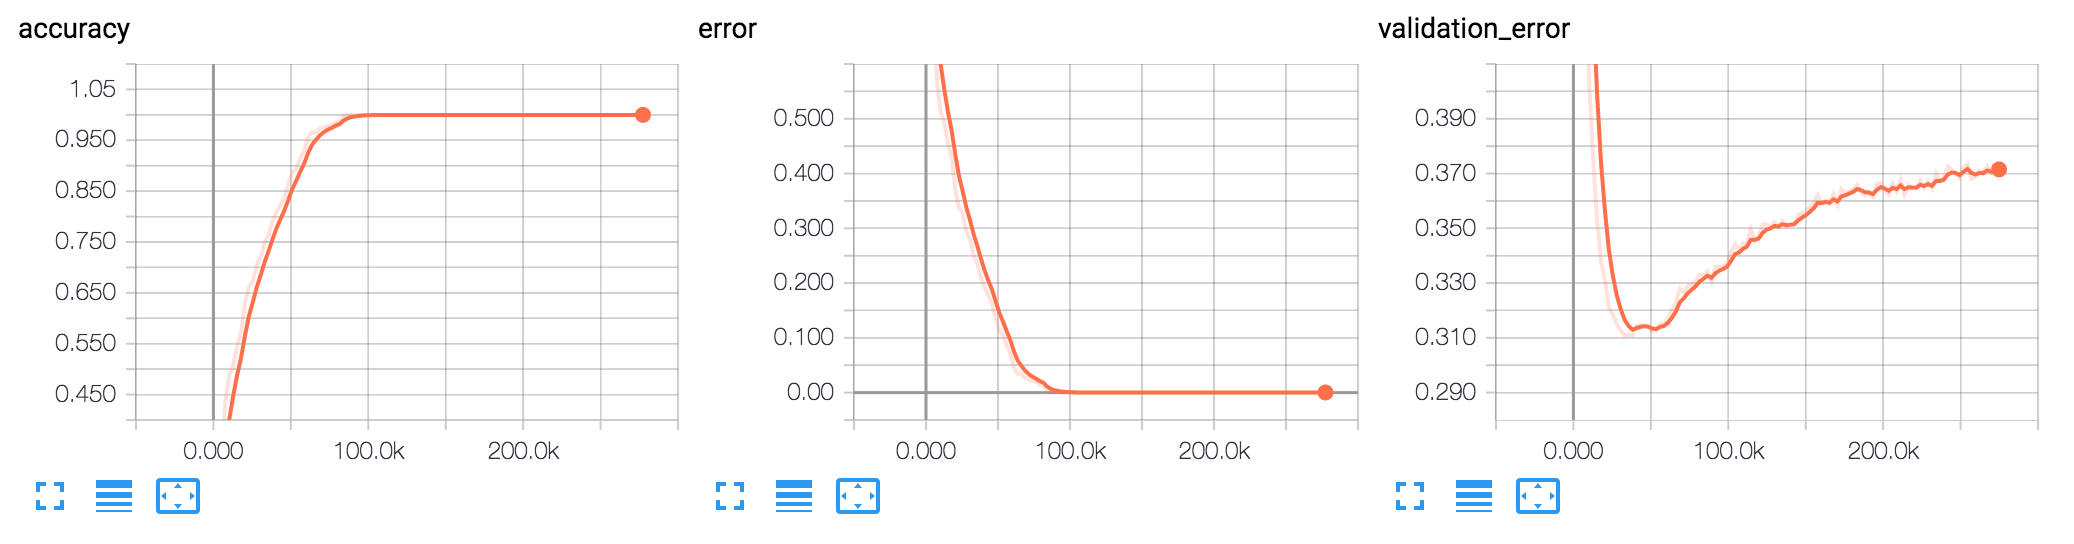
\includegraphics[width=.9\columnwidth]{graphics/rnn_accuracy.png}
	\caption{\label{fig:rnn_accuracy} \footnotesize{training process for the RNN. Training accuracy on the left, error in the centre and validation error on the right.}}
\end{figure} 
In comparison to the originial, however, our results are rather unspectacular. Their accuracy was between 91,5 and 94 percent for the IIT5K data set and even identified very ambiguous pictures.

\section{Conclusion}
%include ideas that could further improve the accuracy, i.e. not train in two steps but in one, use other datasets as well, smaller step sizes for sliding window
%name other papers that are related to this or follow up on it (and what they did better)
The results that we achieved where slightly less impressive than those of the original publication. There are a couple of improvisations that could be done in future research projects that we would like to outline. A first idea would be to train the network not in 2 separate steps but rather as one end-to-end process. This would likely result in better outcomes since the entire CNN would already get information from the RNN and CTC through backpropagation. A second idea is to use a bigger data set of images for training. The IIT5K seems like a good benchmark but due to the test train split overfitting might have occured which might be solved by significantly bigger datasets. A third possibility is to train the CNN and RNN on significantly lower sliding window frame sizes, i.e. 2 instead of 8 %actually we are doing this. 
\\
The paper we are replicating was published in summer 2015 which is already two and a half years back. In a field with such rapid changes like scene recognition other projects have already further improved the methods that were revolutionary then. In the following we would like to have a closer look at some of the new ideas and improvements. \\
%read and cite the followup paper
The first improvements were made by ~\cite{DBLP:journals/corr/abs-1709-01727} who improved the sliding window by constructing the sliding window in a way that more closely resembles the movements of saccades by biological eyes. They also added more layers to the CNN in the first step of the training. Lastly they improve the CTC algorithm to reduce the search space and make training with a beam decoder more effective. In the end they were able to improve accuracy from 94 to 98.9 and 91.5 to 96.7 percent on the IIT5K dataset respectively. 
The second paper by ~\cite{DBLP:journals/corr/TianHHH016} is one conducted by partly the same authors that uses a similar approach to the original but contributed a new method which they call connectionist text proposal network (CTPN). The CTPN essentially is a convolutional network that already detects text structures within bigger image scenes. Due to this new technique they were not only able to find text within natural images, without cutting it out manually as in our paper, but also significantly improve nearly all benchmarks on the ICDAR data sets from 2011, 2013 and 2015.
%find and compare to other approaches
The last paper uses a slightly different approach on the just named ICDAR data sets. In ~\cite{DBLP:journals/corr/HeH0Y15} they only use a text-attentional convolutional neural networks for scene text detection without any recurrent part. They were able to break the benchmark of the ICDAR 2013 data set but were very quickly beaten afterwards by ~\cite{DBLP:journals/corr/TianHHH016} which uses an RNN. This last paper was mainly presented to show that there are were potent methods of classification that do not require a recurrent part out there.\\


\bibliographystyle{alpha}
\bibliography{bibliography}
%https://github.com/chongyangtao/Awesome-Scene-Text-Recognition
%https://arxiv.org/abs/1709.01727 (this is a follow up paper)
%https://arxiv.org/pdf/1601.01100.pdf (same approach for house number recognition)
%http://adsabs.harvard.edu/abs/2016arXiv160105610L (same approach for license plate recognition)

\end{document}
